% !TeX program = lualatex
% !TeX encoding = UTF-8
\documentclass[border=10pt]{standalone}

\usepackage{xcolor}
  \pagecolor{black}
  \color{white}

\usepackage{amsmath}
\usepackage[all]{xy}
\usepackage{tikz-cd}
\usepackage{varwidth}

\begin{document}
\begin{varwidth}{\linewidth}
	\centering

	\section*{Method 1: Using package \texttt{xy}}
	\vspace{0.5cm}

	\centerline{
	\xymatrix{
	& H^{k+1}(M) \ar[r]^<<<<<<<<<<<{i^*} & \cdots \\
	& H^k(M) \ar[r]^>>>>>{i^*}
	& H^k(U) \oplus H^k(V) \ar[r]^>>>>>{j^*}
	& H^k(U \cap V) \ar `[ul] `[l] `[lllu] |{d^*} `[l] [rlllu] \\
	&  *{}  & \cdots \ar[r]^<<<<<<<<<<{j^*}
	& H^{k-1}(U \cap V) \ar `[ul] `[l] `[lllu] |{d^*} `[l] [rlllu]
	}
	}

	\vspace{1cm}
	\hrule
	\vspace{1cm}

	\section*{Method 2: Using package \texttt{tikz-cd}}
	\vspace{0.5cm}

	\tikzset{
		curarrow/.style={
				rounded corners=8pt,
				to path={-- ([xshift=50pt]\tikztostart.center)
						|- (#1) node[fill=black, text=white] {$\scriptstyle d^*$}
						-| ([xshift=-40pt]\tikztotarget.center)
						-- (\tikztotarget)}
			}
	}

	\begin{tikzcd}[cells={nodes={text height=2ex,text depth=0.75ex}}]
		{} & & H^{k+1}(M) \arrow{r}{i^*} & \cdots \\
		{} & & H^k(M) \arrow{r}{i^*} & H^k(U) \oplus H^k(V) \arrow{r}{j^*}
		\arrow[draw=none]{u}[name=Y, shape=coordinate]{}
		\arrow[draw=none]{d}[name=Z,shape=coordinate]{}
		& H^k(U \cap V) \arrow[curarrow=Y]{ull}{} \\
		& & & \cdots \arrow{r}{j^*} & H^{k-1}(U \cap V)
		\arrow[curarrow=Z]{ull}{} \\
	\end{tikzcd}

	\vspace{1cm}
	\hrule
	\vspace{1cm}

	\section*{Method 3: Using package \texttt{tikz}}
	\vspace{0.5cm}

	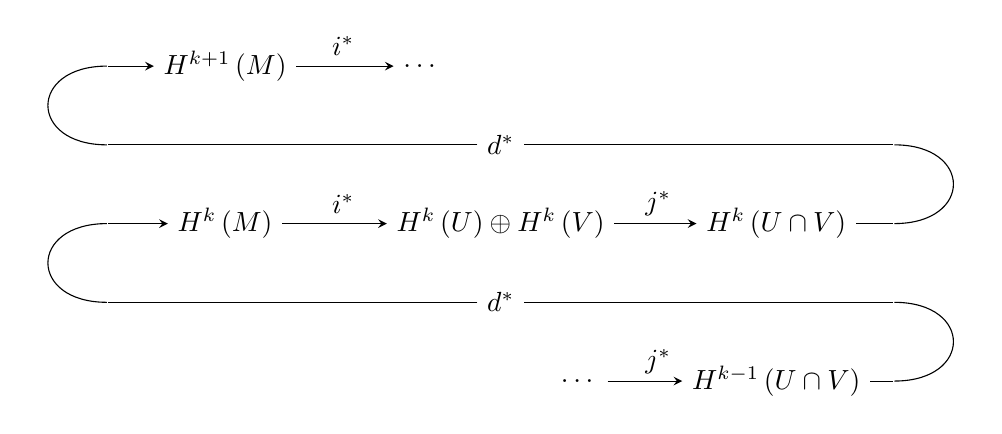
\begin{tikzpicture}
		\tikzstyle{tight}  = [outer sep=0,inner sep=0]
		\tikzstyle{myarr}  = [-stealth]
		\tikzstyle{myline} = [-,tight]
		\node (v1) at (1,0)     {$\dots$};
		\node (v2) at (3.5,0)   {$H^{k-1}\left(U \cap V \right)$};
		\node (v5) at (0,1)     {$d^*$};
		\node (v13) at (0,3)    {$d^*$};
		\node (v8) at (-3.5,2)  {$H^k\left( M \right)$};
		\node (v9) at (0,2)     {$H^k\left( U \right) \oplus H^k\left( V \right)$};
		\node (v10) at (3.5,2)  {$H^{k}\left(U \cap V \right)$};
		\node (v16) at (-3.5,4) {$H^{k+1}\left( M \right)$};
		\node (v17) at (-1,4)   {$\dots$};
		\draw [myline](5,0)  node (v3)  {} .. controls (6,0) and (6,1)   .. (5,1)  node (v4) {};
		\draw [myline](-5,1) node (v6)  {} .. controls (-6,1) and (-6,2) .. (-5,2) node (v7) {};
		\draw [myline](5,2)  node (v11) {} .. controls (6,2) and (6,3)   .. (5,3)  node (v12) {};
		\draw [myline](-5,3) node (v14) {} .. controls (-6,3) and (-6,4) .. (-5,4) node (v15) {};
		\node at (2,0.25) {$j^*$};
		\node at (-2,2.25) {$i^*$};
		\node at (2,2.25) {$j^*$};
		\node at (-2,4.25) {$i^*$};

		\draw [myarr] (v1) edge (v2);
		\draw [myarr] (v7) edge (v8);
		\draw [myarr] (v8) edge (v9);
		\draw [myarr] (v9) edge (v10);
		\draw [myarr] (v15) edge (v16);
		\draw [myarr] (v16) edge (v17);

		\draw [myline] (v2) edge (v3);
		\draw [myline] (v4) edge (v5);
		\draw [myline] (v5) edge (v6);
		\draw [myline] (v10) edge (v11);
		\draw [myline] (v12) edge (v13);
		\draw [myline] (v13) edge (v14);
	\end{tikzpicture}

\end{varwidth}
\end{document}
